%% State Space Modelling of Dynamic Systems
%% Lecture 20: State Feedback Control
\def\FileDate{10/02/02}
\def\FileVersion{1.0}
% ----------------------------------------------------------------
% Notes pages *********************************************************
% ----------------------------------------------------------------

\begin{slide}
   \heading{State Feedback Control}
One of the advantages of state space models is that it is possible to apply state feedback to place the closed loop poles into any desired positions.

\textbf{State Space Design Methodology}

\begin{enumerate}
	\item Design control law to place closed loop poles where desired
	\item If full state not available for feedback, then design an \emph{Observer} to compute the states from the system output
	\item Combine \emph{Observer} and \emph{Controller} -- this takes the place of the \emph{Classical Compensator}
	\item Introduce the \emph{Reference Input} -- affects the closed loop zeros but not the poles making it possible to improve the transient response and tracking accuracy
\end{enumerate}	
\end{slide}

\begin{slide}
   \heading{State Feedback Compensator}
   \begin{center}
   	\resizebox{280pt}{!}{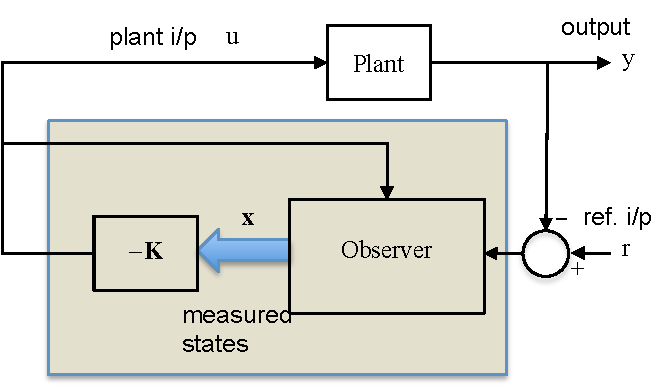
\includegraphics{pictures/statefb.pdf}}
   \end{center}
\end{slide}

\section*{Finding the Control Law} % (fold)
\label{sec:finding_the_control_law}

We shall only consider SISO systems here.


\begin{center}
	\resizebox{200pt}{!}{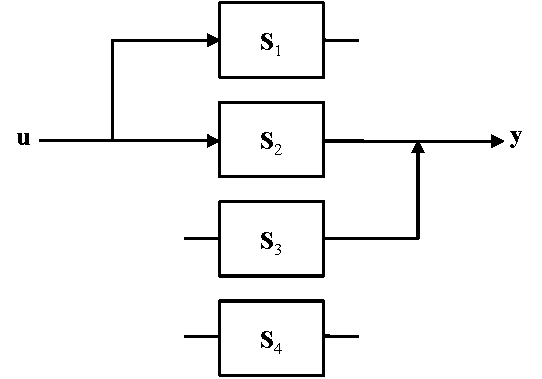
\includegraphics{pictures/partitioning.pdf}}
\end{center}
\endinput

%%% Local Variables: 
%%% mode: latex
%%% TeX-master: "notes"
%%% End:
\ifslidesonly
\begin{slide}
   \heading{Finding the Control Law (1)}
   
\begin{center}
	\resizebox{200pt}{!}{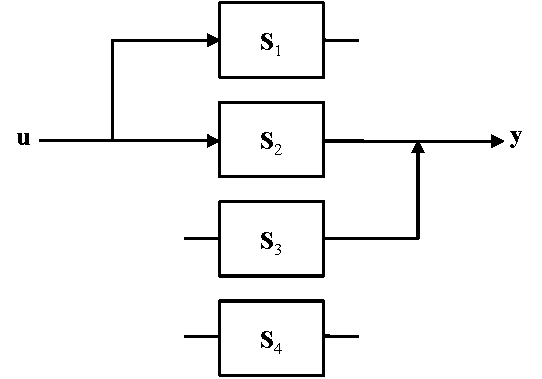
\includegraphics{pictures/partitioning.pdf}}
\end{center}
\endinput

%%% Local Variables: 
%%% mode: latex
%%% TeX-master: "notes"
%%% End:
\end{slide}
\fi

Given the transformation $\mathbf{T}^{-1}\mathbf{AT}=\mathbf{\Lambda}$:
\begin{eqnarray*}
	\mathbf{A}t & = & (\mathbf{T\Lambda T}^{-1}) t \\
	\mathbf{A}^nt^n & = & (\mathbf{T\Lambda T}^{-1})(\mathbf{T\Lambda T}^{-1})\ldots(\mathbf{T\Lambda T}^{-1})t^n \\
	                & = & \mathbf{T\Lambda T}^{-1}\mathbf{T\Lambda T}^{-1}\ldots\mathbf{T\Lambda T}^{-1}t^n \\
	\mathbf{A}^nt^n & = & \mathbf{T\Lambda}\mathbf{I}\mathbf{\Lambda I}\ldots\mathbf{I\Lambda T}^{-1}t^n \\
	\               & = & \mathbf{T\Lambda}^n\mathbf{T}^{-1}t^n \\
\end{eqnarray*}
\endinput

%%% Local Variables: 
%%% mode: latex
%%% TeX-master: "notes"
%%% End:
\ifslidesonly
\begin{slide}
	\heading{Finding the Control Law (2)}
   Given the transformation $\mathbf{T}^{-1}\mathbf{AT}=\mathbf{\Lambda}$:
\begin{eqnarray*}
	\mathbf{A}t & = & (\mathbf{T\Lambda T}^{-1}) t \\
	\mathbf{A}^nt^n & = & (\mathbf{T\Lambda T}^{-1})(\mathbf{T\Lambda T}^{-1})\ldots(\mathbf{T\Lambda T}^{-1})t^n \\
	                & = & \mathbf{T\Lambda T}^{-1}\mathbf{T\Lambda T}^{-1}\ldots\mathbf{T\Lambda T}^{-1}t^n \\
	\mathbf{A}^nt^n & = & \mathbf{T\Lambda}\mathbf{I}\mathbf{\Lambda I}\ldots\mathbf{I\Lambda T}^{-1}t^n \\
	\               & = & \mathbf{T\Lambda}^n\mathbf{T}^{-1}t^n \\
\end{eqnarray*}
\endinput

%%% Local Variables: 
%%% mode: latex
%%% TeX-master: "notes"
%%% End:
\end{slide}
\fi

 
The matrix function becomes:
\begin{eqnarray*}
	f(\mathbf{A}t) & = & f_0\mathbf{TIT}^{-1} + f_1\mathbf{T\Lambda T}^{-1}t + f_2\mathbf{T\Lambda}^2\mathbf{T}^{-1}t^2 + \cdots + f_n\mathbf{T\Lambda}^n\mathbf{T}^{-1}t^n + \cdots \\
	f(\mathbf{A}t) & = & \mathbf{T}\left(f_0\mathbf{I} + f_1\mathbf{\Lambda}t + f_2\mathbf{\Lambda}^2t^2 + \cdots + f_n\mathbf{\Lambda}^nt^n + \cdots \right)\mathbf{T}^{-1}\\
	               & = & \mathbf{T}f(\mathbf{\Lambda}t)\mathbf{T}^{-1}
\end{eqnarray*}
 
The term inside the brackets on the rhs is a diagonal matrix and the $i^\mathrm{th}$ diagonal element is:
\[
f_0+f_1\lambda_it + f_2\lambda_i^2t^2 + \cdots + f_n\lambda_i^nt^ + \cdots
\]
From the Taylor series this must be $f(\lambda_i t)$:
\[
f(\mathbf{A} t)=\mathbf{T} f(\mathbf{\Lambda} t) \mathbf{T}^{-1}
\]   
where $f(\mathbf{\Lambda} t)=\mathrm{diag}\left(f(\lambda_i t)\right)$.

\endinput

%%% Local Variables: 
%%% mode: latex
%%% TeX-master: "notes"
%%% End:
\ifslidesonly
\begin{slide}
	\heading{Finding the Control Law (3)}
   The matrix function becomes:
\begin{eqnarray*}
	f(\mathbf{A}t) & = & f_0\mathbf{TIT}^{-1} + f_1\mathbf{T\Lambda T}^{-1}t + f_2\mathbf{T\Lambda}^2\mathbf{T}^{-1}t^2 + \cdots + f_n\mathbf{T\Lambda}^n\mathbf{T}^{-1}t^n + \cdots \\
	f(\mathbf{A}t) & = & \mathbf{T}\left(f_0\mathbf{I} + f_1\mathbf{\Lambda}t + f_2\mathbf{\Lambda}^2t^2 + \cdots + f_n\mathbf{\Lambda}^nt^n + \cdots \right)\mathbf{T}^{-1}\\
	               & = & \mathbf{T}f(\mathbf{\Lambda}t)\mathbf{T}^{-1}
\end{eqnarray*}
 
The term inside the brackets on the rhs is a diagonal matrix and the $i^\mathrm{th}$ diagonal element is:
\[
f_0+f_1\lambda_it + f_2\lambda_i^2t^2 + \cdots + f_n\lambda_i^nt^ + \cdots
\]
From the Taylor series this must be $f(\lambda_i t)$:
\[
f(\mathbf{A} t)=\mathbf{T} f(\mathbf{\Lambda} t) \mathbf{T}^{-1}
\]   
where $f(\mathbf{\Lambda} t)=\mathrm{diag}\left(f(\lambda_i t)\right)$.

\endinput

%%% Local Variables: 
%%% mode: latex
%%% TeX-master: "notes"
%%% End:
\end{slide}
\fi

The vector $[v_{31}, i_{1}]^T$ is called the ``\emph{state
vector}.'' Its elements are state variables.
\endinput
%%% Local Variables: 
%%% mode: latex
%%% TeX-master: "notes"
%%% End: 

\ifslidesonly
\begin{slide}
	\heading{Finding the Control Law (4)}
   The vector $[v_{31}, i_{1}]^T$ is called the ``\emph{state
vector}.'' Its elements are state variables.
\endinput
%%% Local Variables: 
%%% mode: latex
%%% TeX-master: "notes"
%%% End: 

\end{slide}
\fi



\subsection*{Example 1} % (fold)
\label{sub:example_1}

\textbf{Problem}: Given,
\[
{\bf{\dot x}} = \left[ {\begin{array}{*{20}c}
   { - 4} & 0  \\
   0 & { - 11}  \\
\end{array}} \right]{\bf{x}} + \left[ {\begin{array}{*{20}c}
   1  \\
   { - 1}  \\
\end{array}} \right]u
\]
find the feedback control law which places the closed-loop poles at: $-10\pm j10$.

\textbf{SOLUTION}:
\begin{eqnarray*}
	0 & = & \det \left[ {s{\bf{I}} - {\bf{A}} + {\bf{BK}}} \right] = \det \left\{ {\left. {\left[ {\begin{array}{*{20}c}
	   {s + 4} & 0  \\
	   0 & {s + 11}  \\
	\end{array}} \right] + \left[ {\begin{array}{*{20}c}
	   1  \\
	   { - 1}  \\
	\end{array}} \right]\left[ {\begin{array}{*{20}c}
	   {k_1 } & {k_2 }  \\
	\end{array}} \right]} \right\}} \right. \\
	0 & = & \det \left[ {\begin{array}{*{20}c}
	   {s + 4 + k_1 } & {k_2 }  \\
	   { - k_1 } & {s + 11 - k_2 }  \\
	\end{array}} \right] \\
	0 & = & (s + 4 + k_1 )(s + 11 - k_2 ) - (k_2 )( - k_1 ) \\
	0 & = & (s+4+k_1)(s+11-k_2)+k_1k_2
\end{eqnarray*}
\begin{equation}
	\label{eq:3}
	s^2+(15+k_1-k_2)s+(44+11k_1-4k_2)=0
\end{equation}

Now the desired CE is:
\[
\alpha_c(s)=(s+10-j10)(s+10+j10) = 0
\]
\begin{equation}\label{eq:4}
	s^2+20s+200=0
\end{equation}

Therefore matching coefficients in Eqs. (\ref{eq:3}) and (\ref{eq:4}):
\[
\begin{array}{c}
 s^2 :1 = 1 \to {\rm{OK}} \\ 
 s^1 :15 + k_1  - k_2  = 20 \to k_1  - k_2  = 5 \\ 
 s^0 :44 + 11k_1  - 4k_2  = 200 \to 11k_1  - 4k_2  = 156 \\ 
 \end{array}
\]

 

Solving for the $k$'s:
\[
\left[ {\begin{array}{*{20}c}
   1 & { - 1}  \\
   {11} & { - 4}  \\
\end{array}} \right]\left[ {\begin{array}{*{20}c}
   {k_1 }  \\
   {k_2 }  \\
\end{array}} \right] = \left[ {\begin{array}{*{20}c}
   5  \\
   {156}  \\
\end{array}} \right]
\]
% MathType!MTEF!2!1!+-
% faaagaart1ev2aaaKnaaaaWenf2ys9wBH5garuavP1wzZbqedmvETj
% 2BSbqefm0B1jxALjharqqtubsr4rNCHbGeaGqiVu0Je9sqqrpepC0x
% bbL8FesqqrFfpeea0xe9Lq-Jc9vqaqpepm0xbba9pwe9Q8fs0-yqaq
% pepae9pg0FirpepeKkFr0xfr-xfr-xb9Gqpi0dc9adbaqaaeGaciGa
% aiaabeqaamaabaabaaGcbaWaamWaaeaafaWabeGabaaabaGaam4Aam
% aaBaaaleaacaaIXaaabeaaaOqaaiaadUgadaWgaaWcbaGaaGOmaaqa
% baaaaaGccaGLBbGaayzxaaGaeyypa0ZaaSaaaeaacaaIXaaabaGaey
% OeI0IaaGinaiabgUcaRiaaigdacaaIXaaaamaadmaabaqbamqabiGa
% aaqaaiabgkHiTiaaisdaaeaacaaIXaaabaGaeyOeI0IaaGymaiaaig
% daaeaacaaIXaaaaaGaay5waiaaw2faamaadmaabaqbamqabiqaaaqa
% aiaaiwdaaeaacaaIXaGaaGynaiaaiAdaaaaacaGLBbGaayzxaaGaey
% ypa0ZaaSaaaeaacaaIXaaabaGaaG4naaaadaWadaqaauaadeqaceaa
% aeaacaaIXaGaaG4maiaaiAdaaeaacaaIXaGaaGimaiaaigdaaaaaca
% GLBbGaayzxaaGaeyypa0ZaamWaaeaafaWabeGabaaabaGaaGymaiaa
% iMdacaGGUaGaaGinaiaaiMdacaaIYaGaaGyoaaqaaiaaigdacaaI0a
% GaaiOlaiaaisdacaaIYaGaaGyoaaaaaiaawUfacaGLDbaaaaa!5BC6!
\[
\left[ {\begin{array}{*{20}c}
   {k_1 }  \\
   {k_2 }  \\
\end{array}} \right] = \frac{1}{{ - 4 + 11}}\left[ {\begin{array}{*{20}c}
   { - 4} & 1  \\
   { - 11} & 1  \\
\end{array}} \right]\left[ {\begin{array}{*{20}c}
   5  \\
   {156}  \\
\end{array}} \right] = \frac{1}{7}\left[ {\begin{array}{*{20}c}
   {136}  \\
   {101}  \\
\end{array}} \right] = \left[ {\begin{array}{*{20}c}
   {19.429}  \\
   {14.429}  \\
\end{array}} \right]
\]

 

Therefore the required feedback control law is:
% MathType!MTEF!2!1!+-
% faaagaart1ev2aaaKnaaaaWenf2ys9wBH5garuavP1wzZbqedmvETj
% 2BSbqefm0B1jxALjharqqtubsr4rNCHbGeaGqiVu0Je9sqqrpepC0x
% bbL8FesqqrFfpeea0xe9Lq-Jc9vqaqpepm0xbba9pwe9Q8fs0-yqaq
% pepae9pg0FirpepeKkFr0xfr-xfr-xb9Gqpi0dc9adbaqaaeGaciGa
% aiaabeqaamaabaabaaGcbaGaamyDaiabg2da9iaadkhacqGHsislda
% WadaqaauaadeqabiaaaeaacaaIXaGaaGyoaiaac6cacaaI0aGaaGOm
% aiaaiMdaaeaacaaIXaGaaGinaiaac6cacaaI0aGaaGOmaiaaiMdaaa
% aacaGLBbGaayzxaaGaaCiEaaaa!3DCD!
\[
u = r - \left[ {\begin{array}{*{20}c}
   {19.429} & {14.429}  \\
\end{array}} \right]{\bf{x}}
\]



\textbf{COMMENT}
This matching of coefficients can always be done, though it is tedious for $n>3$, \textbf{EXCEPT} in the case of the \emph{Control Canonical Form}.

% subsection example_1 (end)
 
% section finding_the_control_law (end)

\section*{State Feedback in the Case of the Control Canonical Form} % (fold)
\label{sec:state_feedback_in_the_case_of_the_control_canonical_form}


From previous work the error dynamics are:
\[
\dot{\mathbf{e}} = (\mathbf{A}-\mathbf{LC})\mathbf{e}
\]
Therefore the dynamics of the combined system is:
\[\left[ {\begin{array}{*{20}c}
   {\dot{\mathbf{x}}}  \\
   {\dot{\mathbf{e}}ß}  \\
\end{array}} \right] = \left[ {\begin{array}{*{20}c}
   {\left( {{\bf{A}} - {\bf{BK}}} \right)} & {{\bf{BK}}}  \\
   {\bf{0}} & {\left( {{\bf{A}} - {\bf{LC}}} \right)}  \\
\end{array}} \right]\left[ {\begin{array}{*{20}c}
   {\bf{x}}  \\
   {\bf{e}}  \\
\end{array}} \right] + \left[ {\begin{array}{*{20}c}
   {\bf{B}}  \\
   {\bf{0}}  \\
\end{array}} \right]r
\]
\endinput

%%% Local Variables: 
%%% mode: latex
%%% TeX-master: "notes"
%%% End:
\ifslidesonly
\begin{slide}
	\heading{Control Canonical Form Simplifies Calculation (1)}
   From previous work the error dynamics are:
\[
\dot{\mathbf{e}} = (\mathbf{A}-\mathbf{LC})\mathbf{e}
\]
Therefore the dynamics of the combined system is:
\[\left[ {\begin{array}{*{20}c}
   {\dot{\mathbf{x}}}  \\
   {\dot{\mathbf{e}}ß}  \\
\end{array}} \right] = \left[ {\begin{array}{*{20}c}
   {\left( {{\bf{A}} - {\bf{BK}}} \right)} & {{\bf{BK}}}  \\
   {\bf{0}} & {\left( {{\bf{A}} - {\bf{LC}}} \right)}  \\
\end{array}} \right]\left[ {\begin{array}{*{20}c}
   {\bf{x}}  \\
   {\bf{e}}  \\
\end{array}} \right] + \left[ {\begin{array}{*{20}c}
   {\bf{B}}  \\
   {\bf{0}}  \\
\end{array}} \right]r
\]
\endinput

%%% Local Variables: 
%%% mode: latex
%%% TeX-master: "notes"
%%% End:
\end{slide}
\fi


When the initial conditions of the state-variables are all zero,
this reduces to the transfer matrix model
\begin{equation}\label{eqn:transfer-function}
  \mathbf{Y}=\left[\mathbf{C}\left[s\mathbf{I}-\mathbf{A}\right]^{-1}\mathbf{B}+\mathbf{D}\right]\mathbf{U}
\end{equation}

\endinput

%%% Local Variables: 
%%% mode: latex
%%% TeX-master: "notes"
%%% End: 

When the observer canonical form is not used, then the design of the observer is more difficult. Ackermann's formula can be adapted as follows:
% MathType!MTEF!2!1!+-
% faaagaart1ev2aaaKnaaaaWenf2ys9wBH5garuavP1wzZbqedmvETj
% 2BSbqefm0B1jxALjharqqtubsr4rNCHbGeaGqiVu0Je9sqqrpepC0x
% bbL8FesqqrFfpeea0xe9Lq-Jc9vqaqpepm0xbba9pwe9Q8fs0-yqaq
% pepae9pg0FirpepeKkFr0xfr-xfr-xb9Gqpi0dc9adbaqaaeGaciGa
% aiaabeqaamaabaabaaGcbaGaaCitamaaCaaaleqabaGaamivaaaaki
% abg2da9maadmaabaqbamqabeabaaaabaGaaGimaaqaaiablAcilbqa
% aiaaicdaaeaacaaIXaaaaaGaay5waiaaw2faaiaad+eadaahaaWcbe
% qaaiabgkHiTiaaigdaaaGccqaHXoqydaWgaaWcbaGaam4yaaqabaGc
% caGGOaGaaCyqamaaCaaaleqabaGaamivaaaakiaacMcaaaa!3EF6!
\[
{\bf{L}}^T  = \left[ {\begin{array}{*{20}c}
   0 &  \ldots  & 0 & 1  \\
\end{array}} \right]\mathcal{O}^{ - 1} \alpha _e ({\bf{A}}^T )
\]
$\mathcal{O}$ is the observability matrix:
\[
\mathcal{O}=[\mathbf{C}^T\vdots\mathbf{A}^T\mathbf{C}^T\vdots\cdots\vdots(\mathbf{A}^T)^{n-1}\mathbf{C}^T]
\]
and if $\alpha_e(s)=s^n + \alpha_1s^{n-1}+\cdots+\alpha_n$ then \[\alpha_e(\mathbf{A}^T)=(\mathbf{A}^T)^n + \alpha_1(\mathbf{A}^T)^{n-1}+\cdots+\mathbf{I}\alpha_n.\]
 

Notice that if the system is unobservable, then the matrix inverse $\mathcal{O}^{-1}$ does not exist and we cannot design an observer for this system.


 
 

\endinput

%%% Local Variables: 
%%% mode: latex
%%% TeX-master: "notes"
%%% End:
\ifslidesonly
\begin{slide}
	\heading{Control Canonical Form (2)}
   When the initial conditions of the state-variables are all zero,
this reduces to the transfer matrix model
\begin{equation}\label{eqn:transfer-function}
  \mathbf{Y}=\left[\mathbf{C}\left[s\mathbf{I}-\mathbf{A}\right]^{-1}\mathbf{B}+\mathbf{D}\right]\mathbf{U}
\end{equation}

\endinput

%%% Local Variables: 
%%% mode: latex
%%% TeX-master: "notes"
%%% End: 

\end{slide}
\begin{slide}
	\heading{Control Canonical Form (3)}
   When the observer canonical form is not used, then the design of the observer is more difficult. Ackermann's formula can be adapted as follows:
% MathType!MTEF!2!1!+-
% faaagaart1ev2aaaKnaaaaWenf2ys9wBH5garuavP1wzZbqedmvETj
% 2BSbqefm0B1jxALjharqqtubsr4rNCHbGeaGqiVu0Je9sqqrpepC0x
% bbL8FesqqrFfpeea0xe9Lq-Jc9vqaqpepm0xbba9pwe9Q8fs0-yqaq
% pepae9pg0FirpepeKkFr0xfr-xfr-xb9Gqpi0dc9adbaqaaeGaciGa
% aiaabeqaamaabaabaaGcbaGaaCitamaaCaaaleqabaGaamivaaaaki
% abg2da9maadmaabaqbamqabeabaaaabaGaaGimaaqaaiablAcilbqa
% aiaaicdaaeaacaaIXaaaaaGaay5waiaaw2faaiaad+eadaahaaWcbe
% qaaiabgkHiTiaaigdaaaGccqaHXoqydaWgaaWcbaGaam4yaaqabaGc
% caGGOaGaaCyqamaaCaaaleqabaGaamivaaaakiaacMcaaaa!3EF6!
\[
{\bf{L}}^T  = \left[ {\begin{array}{*{20}c}
   0 &  \ldots  & 0 & 1  \\
\end{array}} \right]\mathcal{O}^{ - 1} \alpha _e ({\bf{A}}^T )
\]
$\mathcal{O}$ is the observability matrix:
\[
\mathcal{O}=[\mathbf{C}^T\vdots\mathbf{A}^T\mathbf{C}^T\vdots\cdots\vdots(\mathbf{A}^T)^{n-1}\mathbf{C}^T]
\]
and if $\alpha_e(s)=s^n + \alpha_1s^{n-1}+\cdots+\alpha_n$ then \[\alpha_e(\mathbf{A}^T)=(\mathbf{A}^T)^n + \alpha_1(\mathbf{A}^T)^{n-1}+\cdots+\mathbf{I}\alpha_n.\]
 

Notice that if the system is unobservable, then the matrix inverse $\mathcal{O}^{-1}$ does not exist and we cannot design an observer for this system.


 
 

\endinput

%%% Local Variables: 
%%% mode: latex
%%% TeX-master: "notes"
%%% End:
\end{slide}
\fi


 
\begin{itemize}
	\item Rule of thumb: observer poles can be faster than the controller poles (i.e. further from the origin) by a factor of 2 to 6. This makes the effect of the observer dynamics short-term and the overall response is dominated by the controller poles.
	\item If noise/disturbance is present this has an effect on the choice:
	\begin{description}
		\item[Process noise $w$:] $d\mathbf{x}/dt=\mathbf{Ax}+\mathbf{B}u+\mathbf{B}_1 w$
		\item[Sensor noise $v$:]  $y = \mathbf{C}x+v$
		\item[Observer:] $d\hat{\mathbf{x}}=\mathbf{A}\hat{\mathbf{x}}+\mathbf{B}u+\mathbf{L}(y-\mathbf{C}\hat{\mathbf{x}})$
		\item[Error $\mathbf{e}=\mathbf{x}-\hat{\mathbf{x}}$:] $d\mathbf{e}/dt=(\mathbf{A}-\mathbf{LC})\mathbf{e}+\mathbf{B}_1 w - \mathbf{L}v.$
	\end{description}
\end{itemize}

\endinput

%%% Local Variables: 
%%% mode: latex
%%% TeX-master: "notes"
%%% End:
\ifslidesonly
\begin{slide}
	\heading{Control Canonical Form (4)}
   \begin{itemize}
	\item Rule of thumb: observer poles can be faster than the controller poles (i.e. further from the origin) by a factor of 2 to 6. This makes the effect of the observer dynamics short-term and the overall response is dominated by the controller poles.
	\item If noise/disturbance is present this has an effect on the choice:
	\begin{description}
		\item[Process noise $w$:] $d\mathbf{x}/dt=\mathbf{Ax}+\mathbf{B}u+\mathbf{B}_1 w$
		\item[Sensor noise $v$:]  $y = \mathbf{C}x+v$
		\item[Observer:] $d\hat{\mathbf{x}}=\mathbf{A}\hat{\mathbf{x}}+\mathbf{B}u+\mathbf{L}(y-\mathbf{C}\hat{\mathbf{x}})$
		\item[Error $\mathbf{e}=\mathbf{x}-\hat{\mathbf{x}}$:] $d\mathbf{e}/dt=(\mathbf{A}-\mathbf{LC})\mathbf{e}+\mathbf{B}_1 w - \mathbf{L}v.$
	\end{description}
\end{itemize}

\endinput

%%% Local Variables: 
%%% mode: latex
%%% TeX-master: "notes"
%%% End:
\end{slide}
\fi

 
\subsection*{Example 2} % (fold)
\label{sub:example_2}

\textbf{Problem}: Given the system TF:
\[
G(s) = \frac{7}{(s+4)(s+11)}
\]
find the control law for the control canonical form which places the closed loop poles at $s=−10\pm j10$.

\textbf{SOLUTION}:
\[
G(s) = \frac{7}{(s+4)(s+11)} = \frac{7}{(s^2+15s+44)}
\]
 
The control canonical form has matrices:
\[
{\bf{A}} = \left[ {\begin{array}{*{20}c}
   { - 15} & { - 44}  \\
   1 & 0  \\
\end{array}} \right];\quad {\bf{B}} = \left[ {\begin{array}{*{20}c}
   1  \\
   0  \\
\end{array}} \right];\quad {\bf{C}} = \left[ {\begin{array}{*{20}c}
   0 & 7  \\
\end{array}} \right];\quad {\bf{D}} = 0
\]
 
\textbf{NB}:  $\mathbf{C}$ is obtained from the TF numerator $(0s+7)$.
so:    
\[
{\bf{A}} - {\bf{BK}} = \left[ {\begin{array}{*{20}c}
   { - 15 - k_1 } & { - 44 - k_2 }  \\
   1 & 0  \\
\end{array}} \right]
\]
and the closed loop CE is:
\begin{equation}
	s^2+(15+k_1)s+(44+k_2)=0 \label{eq:7}
\end{equation}
The desired CE is:
\[
\alpha_c(s)=(s+10-j10)(s+10+j10) = 0
\]
\begin{equation}\label{eq:8}
	s^2+20s+200=0
\end{equation}
 
Comparing Eqs. (\ref{eq:7})  and  (\ref{eq:8}) gives:
% MathType!MTEF!2!1!+-
% faaagaart1ev2aaaKnaaaaWenf2ys9wBH5garuavP1wzZbqedmvETj
% 2BSbqefm0B1jxALjharqqtubsr4rNCHbGeaGqiVu0Je9sqqrpepC0x
% bbL8FesqqrFfpeea0xe9Lq-Jc9vqaqpepm0xbba9pwe9Q8fs0-yqaq
% pepae9pg0FirpepeKkFr0xfr-xfr-xb9Gqpi0dc9adbaqaaeGaciGa
% aiaabeqaamaabaabaaGcbaGaaGymaiaaiwdacqGHRaWkcaWGRbWaaS
% baaSqaaiaaigdaaeqaaOGaeyypa0JaaGOmaiaaicdacqGHsgIRcaWG
% RbWaaSbaaSqaaiaaigdaaeqaaOGaeyypa0JaaGynaaaa!3A5E!
\[
15 + k_1  = 20 \to k_1  = 5
\]
and
% MathType!MTEF!2!1!+-
% faaagaart1ev2aaaKnaaaaWenf2ys9wBH5garuavP1wzZbqedmvETj
% 2BSbqefm0B1jxALjharqqtubsr4rNCHbGeaGqiVu0Je9sqqrpepC0x
% bbL8FesqqrFfpeea0xe9Lq-Jc9vqaqpepm0xbba9pwe9Q8fs0-yqaq
% pepae9pg0FirpepeKkFr0xfr-xfr-xb9Gqpi0dc9adbaqaaeGaciGa
% aiaabeqaamaabaabaaGcbaGaaGymaiaaiwdacqGHRaWkcaWGRbWaaS
% baaSqaaiaaigdaaeqaaOGaeyypa0JaaGOmaiaaicdacqGHsgIRcaWG
% RbWaaSbaaSqaaiaaigdaaeqaaOGaeyypa0JaaGynaaaa!3A5E!
\[
44 + k_2  = 200 \to k_2  = 156
\]
giving the control law as:   
\[
u = r - \left[ {\begin{array}{*{20}c}
   {5} & {156}  \\
\end{array}} \right]{\bf{x}}
\]

% subsection example_2 (end)Given the system TF:


% section state_feedback_in_the_case_of_the_control_canonical_form (end)

\section*{A Transfer Function Model of State Feedback} % (fold)
\label{sec:a_transfer_function_model_of_state_feedback}

The last example had a system TF with no zeros. In this case it is easy to construct the equivalent classical controller. We had the feedback law:
\[
u=r-5x_1-156x_2
\]

Now $y=7x_2$ and $\dot{x}_2=x_1$ therefore $X_2(s)=Y(s)/7$ and $X_1(s)=sX_2(s)=sY(s)/7$. Therefore
\begin{eqnarray*}
	U(s) & = & R(s)-rX_1(s)-156X_2(s) \\
	& = & R(s) - \frac{1}{7}(5s+156)Y(s)
\end{eqnarray*}

\endinput

%%% Local Variables: 
%%% mode: latex
%%% TeX-master: "notes"
%%% End:
\ifslidesonly
\begin{slide}
	\heading{Transfer Function Model of State Feedback (1)}
   The last example had a system TF with no zeros. In this case it is easy to construct the equivalent classical controller. We had the feedback law:
\[
u=r-5x_1-156x_2
\]

Now $y=7x_2$ and $\dot{x}_2=x_1$ therefore $X_2(s)=Y(s)/7$ and $X_1(s)=sX_2(s)=sY(s)/7$. Therefore
\begin{eqnarray*}
	U(s) & = & R(s)-rX_1(s)-156X_2(s) \\
	& = & R(s) - \frac{1}{7}(5s+156)Y(s)
\end{eqnarray*}

\endinput

%%% Local Variables: 
%%% mode: latex
%%% TeX-master: "notes"
%%% End:
\end{slide}
\fi

\[
s{\bf{\hat X}}(s) =  {\bf{A\hat X}}(s) + {\bf{B}}U(s) + {\bf{L}}\left( {Y(s) - {\bf{C\hat X}}}(s) \right)
\]
then,
\[
\left( {s{\bf{I}} - {\bf{A}} + {\bf{LC}}} \right){\bf{\hat X}}(s) = {\bf{B}}U(s) + {\bf{L}}Y(s) 
\]
or,
\[
{\bf{\hat X}}(s) = {\bf{M}}^{ - 1} {\bf{B}}U(s) + {\bf{M}}^{ - 1} {\bf{L}}Y(s)
\]


\endinput

%%% Local Variables: 
%%% mode: latex
%%% TeX-master: "notes"
%%% End:
\ifslidesonly
\begin{slide}
	\heading{Transfer Function Model of State Feedback (2)}
   \[
s{\bf{\hat X}}(s) =  {\bf{A\hat X}}(s) + {\bf{B}}U(s) + {\bf{L}}\left( {Y(s) - {\bf{C\hat X}}}(s) \right)
\]
then,
\[
\left( {s{\bf{I}} - {\bf{A}} + {\bf{LC}}} \right){\bf{\hat X}}(s) = {\bf{B}}U(s) + {\bf{L}}Y(s) 
\]
or,
\[
{\bf{\hat X}}(s) = {\bf{M}}^{ - 1} {\bf{B}}U(s) + {\bf{M}}^{ - 1} {\bf{L}}Y(s)
\]


\endinput

%%% Local Variables: 
%%% mode: latex
%%% TeX-master: "notes"
%%% End:
\end{slide}
\fi



% section a_transfer_function_model_of_state_feedback (end)

\section*{Ackermann's Formula} % (fold)
\label{sec:ackermann_s_formula}

\subsection*{State Feedback Design for any Form of State Space Model} % (fold)
As stated previously, the derivation of the feedback law is tedious for systems of order  $n>3$  except in the case of the controller canonical form. One approach to the problem is to transform the given model to controller canonical form, derive the control law in terms of these states and then transform back to the original system. Ackermann derived the following formula by this method.
\ifslidesonly
\begin{slide}
   \heading{State Feedback Design for any Form of State Space Model}
\begin{itemize}
	\item As stated previously, the derivation of the feedback law is tedious for systems of order  $n>3$  except in the case of the controller canonical form.
	\item One approach to the problem is to transform the given model to controller canonical form, derive the control law in terms of these states and then transform back to the original system.
	\item Ackermann derived the following formula by this method.
\end{itemize}
\end{slide}
\fi

\subsection*{The formula} % (fold)
\label{sub:the_formula}

Now
\[
U(s) =  - {\bf{K\hat X}}(s) 
\]
so
\[
U (s) =   - {\bf{K}}\left( {{\bf{M}}^{ - 1} {\bf{B}}U(s) + {\bf{M}}^{ - 1} {\bf{L}}Y(s)} \right) 
\]
\[
 \left( {1 + {\bf{KM}}^{ - 1} {\bf{B}}} \right)U(s) =  - {\bf{KM}}^{ - 1} {\bf{L}}Y(s)
\]

\[ 
H\left( s \right) =  - \frac{U(s)}{Y(sßß)} = \frac{{{\bf{KM}}^{ - 1} {\bf{L}}}}{{1 + {\bf{KM}}^{ - 1} {\bf{B}}}} 
\]




\endinput

%%% Local Variables: 
%%% mode: latex
%%% TeX-master: "notes"
%%% End:
\ifslidesonly
\begin{slide}
	\heading{Ackermann's Formula}
   Now
\[
U(s) =  - {\bf{K\hat X}}(s) 
\]
so
\[
U (s) =   - {\bf{K}}\left( {{\bf{M}}^{ - 1} {\bf{B}}U(s) + {\bf{M}}^{ - 1} {\bf{L}}Y(s)} \right) 
\]
\[
 \left( {1 + {\bf{KM}}^{ - 1} {\bf{B}}} \right)U(s) =  - {\bf{KM}}^{ - 1} {\bf{L}}Y(s)
\]

\[ 
H\left( s \right) =  - \frac{U(s)}{Y(sßß)} = \frac{{{\bf{KM}}^{ - 1} {\bf{L}}}}{{1 + {\bf{KM}}^{ - 1} {\bf{B}}}} 
\]




\endinput

%%% Local Variables: 
%%% mode: latex
%%% TeX-master: "notes"
%%% End:
\end{slide}
\fi

$\mathcal{C}$ is the controllability matrix (see Lecture 19):
\[
\mathcal{C} = [\mathbf{B}\vdots\mathbf{AB}\vdots\cdots\vdots\mathbf{A}^{n-1}\mathbf{B}]
\]
and
\[
\alpha_c(\mathbf{A})=\mathbf{A}^n + \alpha_1\mathbf{A}^{n-1}+ \cdots + \alpha_n\mathbf{I}
\]

\endinput

%%% Local Variables: 
%%% mode: latex
%%% TeX-master: "notes"
%%% End:
\ifslidesonly
\begin{slide}
	\heading{Explanation of the Terms}
   $\mathcal{C}$ is the controllability matrix (see Lecture 19):
\[
\mathcal{C} = [\mathbf{B}\vdots\mathbf{AB}\vdots\cdots\vdots\mathbf{A}^{n-1}\mathbf{B}]
\]
and
\[
\alpha_c(\mathbf{A})=\mathbf{A}^n + \alpha_1\mathbf{A}^{n-1}+ \cdots + \alpha_n\mathbf{I}
\]

\endinput

%%% Local Variables: 
%%% mode: latex
%%% TeX-master: "notes"
%%% End:
\end{slide}
\fi

\[
u = r - \mathbf{K}\hat{\mathbf{x}}
\]
Taking Laplace transforms
\[
U = R - \mathbf{K}\hat{\mathbf{X}}
\]

\endinput

%%% Local Variables: 
%%% mode: latex
%%% TeX-master: "notes"
%%% End:
\ifslidesonly
\begin{slide}
	\heading{Caveats}
   \[
u = r - \mathbf{K}\hat{\mathbf{x}}
\]
Taking Laplace transforms
\[
U = R - \mathbf{K}\hat{\mathbf{X}}
\]

\endinput

%%% Local Variables: 
%%% mode: latex
%%% TeX-master: "notes"
%%% End:
\end{slide}
\fi

\subsection*{Matlab Function}
\[
U=R-\mathbf{K}\left(\mathbf{M}^{-1}\mathbf{B}U + \mathbf{M}^{-1}{\bf{L}}Y\right)
\]
Re-arranging:
\[
\left(\mathbf{KM}^{-1}\mathbf{B}+1\right)U=R-\mathbf{KM}^{-1}\mathbf{L}Y
\]
therefore,
\[
U=\frac{1}{\mathbf{KM}^{-1}\mathbf{B}+1}R-\frac{\mathbf{KM}^{-1}\mathbf{L}}{\mathbf{KM}^{-1}\mathbf{B}+1}Y
\]

\endinput

%%% Local Variables: 
%%% mode: latex
%%% TeX-master: "notes"
%%% End:
\ifslidesonly
\begin{slide}
	\heading{Matlab Function}
   \[
U=R-\mathbf{K}\left(\mathbf{M}^{-1}\mathbf{B}U + \mathbf{M}^{-1}{\bf{L}}Y\right)
\]
Re-arranging:
\[
\left(\mathbf{KM}^{-1}\mathbf{B}+1\right)U=R-\mathbf{KM}^{-1}\mathbf{L}Y
\]
therefore,
\[
U=\frac{1}{\mathbf{KM}^{-1}\mathbf{B}+1}R-\frac{\mathbf{KM}^{-1}\mathbf{L}}{\mathbf{KM}^{-1}\mathbf{B}+1}Y
\]

\endinput

%%% Local Variables: 
%%% mode: latex
%%% TeX-master: "notes"
%%% End:
\end{slide}
\fi

% subsection the_formula (end)
 
eg. Given:
 
find the feedback vector K to place the closed loop poles at s = −1 , −1 using Ackermann's formula.
Answer
 
 
 
 
Add 3 x row1 to row2 then:  -9v2=1, and v1=2v2  
 

 
Effect of State Feedback on the Closed Loop Zeros
Since,
 

then the closed loop system is:

 

By analogy with previous work, the TF from input  r  to output  y  is:

 

 
The closed loop TF zeros are determined by the numerator determinant.

Adding K times the 2nd column to the first cancels terms whilst leaving the determinant unchanged.

The new form for the TF is:

 

Notice now that numerator is identical to that of the open loop TF.

This implies that the state feedback control has left the open loop zeros unchanged.

The different denominator is due to the feedback action which alters the pole positions as required.
 
Effect of Zero Locations on the Feedback Gains

When a zero is close to a pole in the TF there is a marked increase in the feedback gains. This effect is best illustrated with an example:

Given a system with a TF,
 
find the control law to move the pole to  pc.

Using the observer canonical form,
 
Design the feedback to move the closed loop pole to pc.
Now,
 
Comparing the constant:
 
 
Notice that the feedback gain  k1  is large if:
(i)	the zero is close to the pole:    z≈p
(ii)	the closed loop pole pc   is far from  p

Therefore, large feedback control gains are required if:

(i)	there exist almost cancelling pole-zero pairs in the open loop TF, making the system almost uncontrollable.







(Notice that in this condition the input  u  is almost disconnected from the integrator for the state.)

(ii)	one tries to move the poles a long way,
 .  This imposes a practical limit on how arbitrarily the poles can be placed. You cannot make a slow system fast without using large gains requiring powerful, expensive actuators to force the plant response. Indeed, excessively large forces may destroy the plant.
 
Pole Selection for Good Design

Large control gains (large values in K) are to be avoided since they result in high energy costs and require high power/bandwidth actuators.

A compromise must be achieved between good system response and control effort.

Sensible choices of poles may be obtained from standard tables which optimise the step response in some way.

e.g. The ITAE (Integral Time and Absolute Error) poles are designed to minimise,
 
These have overshoot. If this is really unacceptable (e.g. in machine tools) then Bessel polynomials can be used.


Order/Type	ITAE	Bessel
1	 
 
2	 
 
3	 
 
etc.	etc.	etc.

 
The above are normalised to give  . To obtain polynomials for  , replace   in the above with  .

e.g.  , the 2nd order ITAE polynomial is:
 

Comments

•	In general the Bessel polynomials have too much damping for normal applications – it is preferable to use ITAE (or Butterworth) poles if some overshoot is acceptable.

•	If zeros are present they tend to "sharpen up" the transient response (faster rise times but consequently with more overshoot). In such cases it may be desirable to place a closed loop pole on top of a troublesome zero and work with the reduced order system as above.

•	The poles closest to the origin matter most; other poles give rise to shorter-term transients only and may need only to be shifted to a better damped location, if necessary, at a similar frequency (distance from the origin).
 
•	A most effective technique is to use optimal control to achieve a compromise between control effort, u, and error, z.

i.e. Find the feedback vector K such as to minimise,
 

where the choice of the parameter k determines the required compromise between,

High Accuracy for High Control Effort
                  (use a large value for k)

Lower Accuracy for Reduced Control Effort
                  (use a smaller value for k)




% section ackermann_s_formula (end)

%----------------------------------------------------------------
% The end of notes
% ----------------------------------------------------------------
\endinput

%%% Local Variables: 
%%% mode: latex
%%% TeX-master: t
%%% End: 
